\section{Programmiersprachen}


\begin{frame}{Java und die JVM}
    \begin{columns}
        \begin{column}{.5\framewidth}
            Java, Kotlin, Clojure, Scala
        \end{column}
        \begin{column}{.4\framewidth}
            
\includegraphics[width=2cm]{resources/logos/java}
        \end{column}
    \end{columns}
\end{frame}

\begin{frame}{C\# und das .NET Framework}
    \begin{columns}
        \begin{column}{.5\framewidth}

        \end{column}
        \begin{column}{.4\framewidth}
            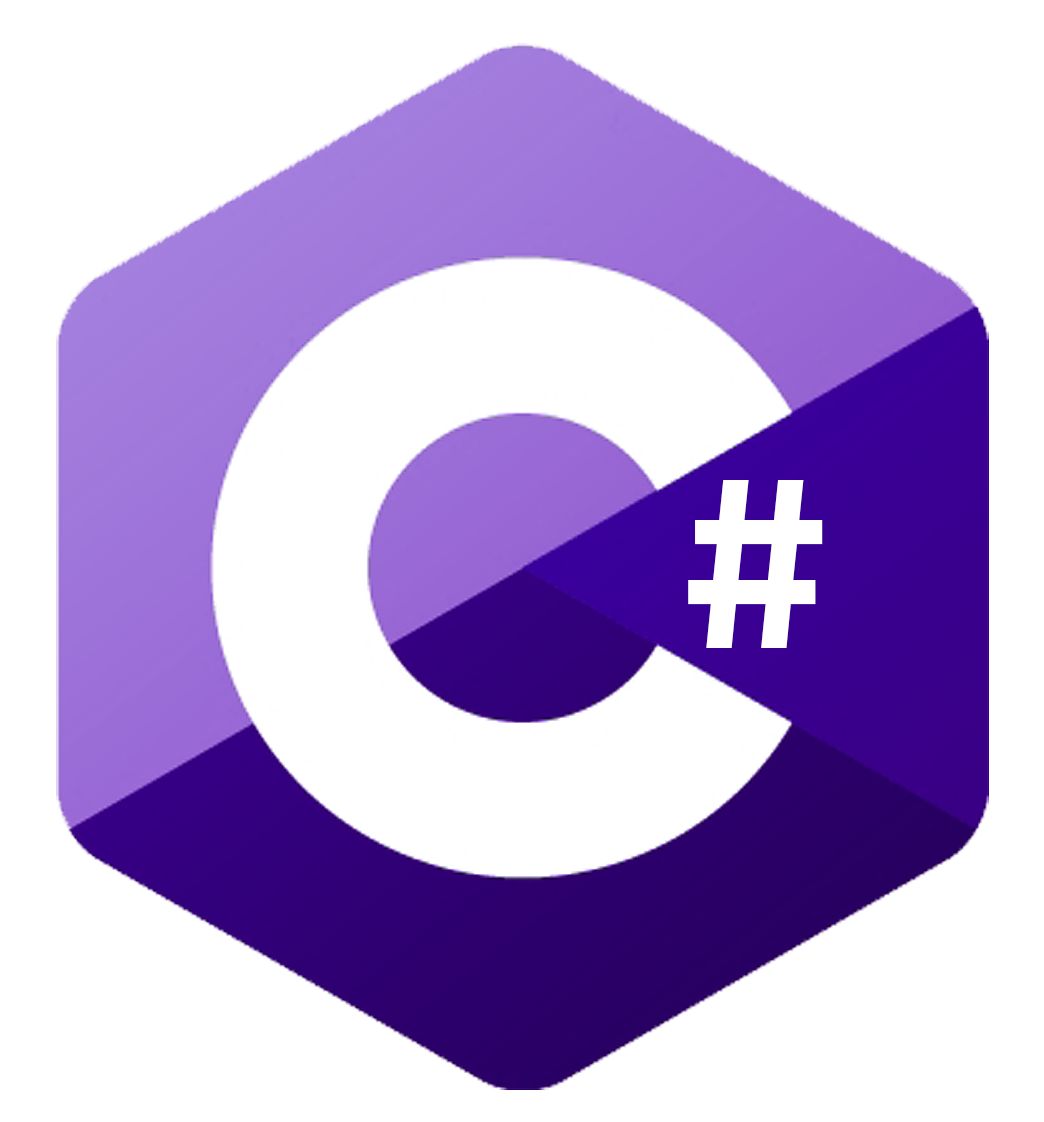
\includegraphics[width=2cm]{resources/logos/csharp}
        \end{column}
    \end{columns}
\end{frame}

\begin{frame}{Python}
    \begin{columns}
        \begin{column}{.5\framewidth}

        \end{column}
        \begin{column}{.4\framewidth}
            
\includegraphics[width=2cm]{resources/logos/python}
        \end{column}
    \end{columns}
\end{frame}